\documentclass[a4paper, 12pt]{article}
\usepackage{graphicx}
\usepackage{mathtools}
\usepackage{color}
\usepackage{epstopdf}
\usepackage[UTF8]{ctex}
\usepackage{listings} 
\usepackage{xcolor}
\usepackage{courier} % 可选,使用Courier字体,类似Jupyter中的代码字体  
  
\lstset{  
    basicstyle=\ttfamily\small, % 设置基本字体样式和大小  
    keywordstyle=\color{blue}, % 设置关键字样式  
    stringstyle=\color{red}, % 设置字符串样式  
    commentstyle=\color{green}, % 设置注释样式  
    breakatwhitespace=false, % 不在空白处自动换行  
    breaklines=true, % 允许自动换行  
    captionpos=b, % 将标题放在底部  
    frame=single, % 为代码块添加单线框(可选)  
    numbers=left, % 在左侧显示行号  
    numberstyle=\tiny\color{gray}, % 设置行号样式  
    tabsize=4, % 设置制表符宽度为4个空格  
    showstringspaces=false, % 不在字符串中显示空格标记  
    language=Python, % 设置语言为Python  
}  
\begin{document}
    {\huge\title{实验报告}}
    {\large\author{程传哲}}
    \date{\today}
    \maketitle
\section{学习成果}

\subsection{命令行环境}
\begin{enumerate}
  \item {\large 中断执行任务结束进程} 
    \begin{itemize}
      \item 
      shell会使用unix提供的信号机制执行进程间的通信 \\
      我们可以使用CTRL-C来停止任务的进程\\
      但有时候SIGNIT信号被捕获无法停止进程\\
      这个时候可以通过CTRL-/实现程序进程中断
    \end{itemize}
  \item {\large 终端执行程序暂停与后台执行}
    \begin{itemize}
      \item 
      SIGSTOP信号可以使进程暂停,在Linux shell中输入CTRL-Z可以发送该信号 \\
      使用fg与bg命令可以回复暂停的工作任务,前台进行或后台进行 \\
    \end{itemize}
  \item {\large tmux终端多路复用器}
    \begin{itemize}
      \item 终端多路复用器分割窗口
      \item tmux多线路有多种指令
      \item {}
        \begin{itemize}
            \item -tmux开始新会话
            \item -tmux new -s name以一个固定名字开始一个会话
            \item -tmux ls 列出当前所有会话
            \item -tmux -a 连接到最后一个会话 -t或指定会话
            \item -\textless C-b \textgreater c 创建一个新的窗口
            \item -\textless C-b \textgreater N 跳转到第N个窗口
            \item -\textless C-b \textgreater p 切换到前一个窗口
            \item -\textless C-b \textgreater n 切换到下一个窗口
            \item -\textless C-b \textgreater w 列出当前所有窗口
        \end{itemize}
    \end{itemize}
  \item{\large 设置别名}
    \begin{itemize}
      \item alias的使用
      \begin{itemize}  
            \item alias la = "ls -a"
            \item unalias la 禁用la
            \item alias ll 获取别名定义
      \end{itemize}
    \end{itemize}
  \item{\large Dotfiles配置文件}
    \begin{itemize}
      \item 对于很对隐藏文件他们不会被ls显示因为他们的开头以点命名
      \item 对于bash来说可以通过编辑\.bashr或是\.bash\
      \_profile来进行配置
      \item 很多情况下需要包含PATH的一些指令以便这些程序被shell找到
    \end{itemize}
  \item{\large SSH远端设备}
    \begin{itemize}
      \item 连接到远端服务器
      \begin{itemize}
            \item 通过URL指定登录ssh name@xxxx.com 
            \item 痛过ip地址指定登录name@xxx.xxx.x.xx
      \end{itemize}
    \end{itemize}
  \item{\large 生成ssh密钥}
    \begin{itemize}
      \item ssh-keygen -o -a 100 -t ed25519 -f \~/.ssh/id\_ed25519
      \item ssh-keygen -t rsa -C "***@gmail.com"通过这些指令可以生成一对密钥分别为私钥与公钥
    \end{itemize}
  \item{\large ssh复制文件}
    \begin{itemize}
      \item scp filename username@ip\_address\:/home/username 但scp现在已经被弃用
      \item rsync username@ip\_address\:/home/username/filename . 使用rsync不仅可以复制文件并且可以复制整个目录
      \item ssh + tee cat localfile | ssh remote\_server tee serverfile将其标准输出到另一个文件
    \end{itemize}  
\item{\large ssh配置}
    \begin{itemize}
      \item 设置别名:alias my\_server= ssh -i \~/\.id\_ed25519 --port 2222 -L 9999\:localhost\:8888 foobar@remote\_server
      \item config设置
      \begin{itemize}
         \item 
         Host vm \\
            \begin{itemize}
            \item{ } User foobar \\ 
            \item{ } HostName 172.16.174.141 \\ 
            \item{ } Port 2222 \\ 
            \item{ } IdentityFile \~/\.ssh/id\_ed25519 \\ 
            \item{ } LocalForward 9999 localhost\:8888  \\ 
            \end{itemize}
      \end{itemize}
    \end{itemize}  
\end{enumerate}
\subsection{python的基本使用}
\begin{enumerate}
\item{\large print}
  \begin{itemize}
    \item print打印语句
  \end{itemize}
\item{\large if else 语句}
      \begin{lstlisting}
        num = 5      
        if num == 3:            
            print 'boss'        
        elif num == 2:
            print 'user'
        elif num == 1:
            print 'worker'
        elif num < 0:           
            print 'error'
        else:
            print 'roadman'     
      \end{lstlisting}
\item{\large while 语句}
    \begin{lstlisting}
      count = 0
      while (count < 9):
        print 'The count is:', count
        count = count + 1
      print "Good bye!"
    \end{lstlisting}
\item {\large for 循环}
    \begin{lstlisting}
      for num in range(10,20):  
        for i in range(2,num): 
            if num%i == 0:      
                j=num/i          
                print ('%d = %d * %d' % (num,i,j))
                break            
            else:                  
                print ('%d is primer number' % num)
    \end{lstlisting}
\item {\large continue语句}
    \begin{lstlisting}
    for letter in 'Python':     
        if letter == 'h':
            continue
        print 'now :', letter
    \end{lstlisting}
\item {\large pass语句}
    \begin{itemize}
        \item python pass语句是空语句,是为了保持程序结构的完整性
    \end{itemize}
    \begin{lstlisting}
    for letter in 'Python':
        if letter == 'h':
            pass
            print 'this is pass'
        print 'now letter :', letter
    \end{lstlisting}
\item {\large 列表}
    \begin{itemize}
        \item 序列都可以进行的操作包括索引,切片,加,乘,检查成员
    \end{itemize}
    \begin{lstlisting}
list01 = ['runoob', 786, 2.23, 'john', 70.2]
list02 = [123, 'john']

print list01
print list02

print list01[0]
print list01[-1]
print list01[0:3]


print list01 * 2


print list01 + list02

print len(list01)


del list02[0]
print list02


print 'john' in list02  # True


for i in list01:
    print i


print cmp(list01, list02)


print max([0, 1, 2, 3, 4])
print min([0, 1])


aTuple = (1,2,3,4)
list03 = list(aTuple)
print list03


list03.append(5)
print list03


list03.extend(list01)
print list03


print list03.count(1)


print list03.index('john')


list03.insert(0, 'hello')
print list03


print list03.pop(0)
print list03


list03.remove(1)
print list03


list03.reverse()
print list03


list03.sort()
print list03
    \end{lstlisting}
\item {\large 模块}
    \begin{itemize}
        \item 导入模块import support等
    \end{itemize}
\item {\large 函数}
    \begin{lstlisting}
def functionname( parameters ):
   function_suite
   return [expression]        
    \end{lstlisting}
\end{enumerate}
\subsection{pyhton视觉}
\begin{enumerate}
\item{\large 基本画图}
    \begin{lstlisting}
from PIL import Image
from pylab import *

im = array(Image.open('1.jpg').convert('L'))

x = [100, 200, 300, 400]
y = [100, 300, 400, 200]
plot(x, y, 'r*')
plot(x[:2], y[:2])
title('yuandonglin')
    \end{lstlisting}
    \begin{figure}[htbp]
        \centering
        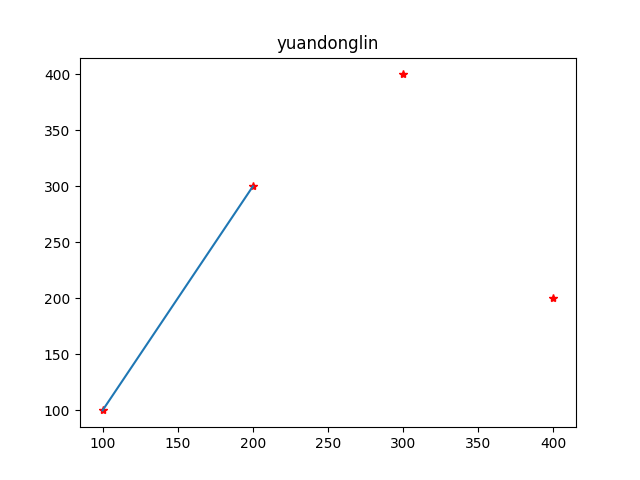
\includegraphics[scale=0.5]{Figure_1.png}
        \caption{figure title}
        \label{figure}
      \end{figure}
\item{\large 处理图像}
    \begin{lstlisting}
from PIL import Image
from pylab import *

im = array(Image.open('1.jpg').convert('L'))

figure()
contour(im, origin='image')
axis('equal')
axis('off')
figure()
hist(im.flatten(), 128)
show()

    \end{lstlisting}
 \begin{figure}[htbp]
        \centering
        
\includegraphics[scale=0.5]{Figure_2.png}
        \caption{figure title}
        \label{figure}
 \end{figure}   
 \begin{figure}[htbp]
        \centering
        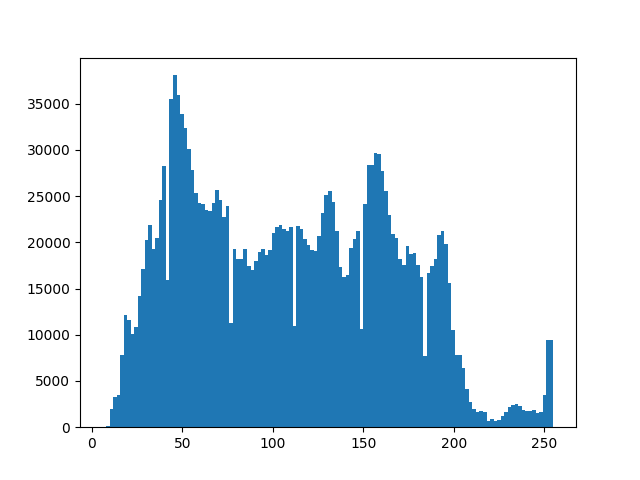
\includegraphics[scale=0.5]{Figure_3.png}
        \caption{figure title}
        \label{figure}
 \end{figure}
\item{\large 输入读取语句}
    \begin{itemize}
        \item read num 回车即可操作
        \item read -p "请输入num的值 " num 其中加入-p可以同时显示与读取
    \end{itemize}
\item{\large 只读变量}
    \begin{itemize}
        \item readonly num = 10回车即可操作 后续将无法通过赋值语句改变num的量
    \end{itemize}
\end{enumerate}
\section{Github链接}
https://github.com/Chengchuanzhe/-.git
\section{学习感悟}
    在本次的系统工具开发实践课中我受益颇多,在深入学习Shell与Vim的过程中,我经历了从初识的困惑到逐渐熟练运用的转变,这一过程不仅提升了我的技术能力,也让我对编程和命令行操作有了更深的理解和感悟,在学习shell中逐渐的了解了各个指令的用处以及shell脚本的使用,在vim的学习中学会了如何去使用vim键盘以及编写程序,这次的课程使我收益匪浅,也会继续在系统操作中继续学习下去
\end{document} 